\chapter*{Le jeu de Nim}

Voici un premier petit jeu simple, pour rentrer dans le sujet. On dispose sur
une table \textit{16 objets}. Chacun leur tour, les deux joueurs ramassent
\textit{un, deux ou trois objets} sur la table. Le joueur qui \textbf{ramasse le
  dernier objet} remporte la partie.

\bigskip
 
\encart{Matériel}{
  \begin{itemize}
    \item 16 petits objets (clous, allumettes{\ldots}  peu importe !)
  \end{itemize}
}

\bigskip
\bigskip
\bigskip

\begin{center}
\newcommand\red[1]{
  \node [circle,fill=red,text=black] {\textbf #1}
}

\newcommand\blue[1]{
  \node [circle,fill=blue,text=white] {\textbf #1};
}

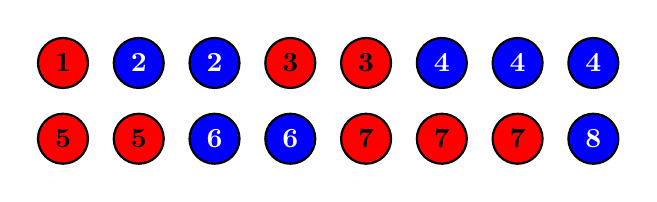
\begin{tikzpicture}

\matrix (m) [nodes={draw, thick}, row sep=0.3cm, column sep=0.3cm] {
  \red{1}; &
  \blue{2}; &
  \blue{2}; &
  \red{3}; &
  \red{3}; &
  \blue{4}; &
  \blue{4}; &
  \blue{4}; \\
  \red{5}; &
  \red{5}; &
  \blue{6}; &
  \blue{6}; &
  \red{7}; &
  \red{7}; &
  \red{7}; &
  \blue{8}; \\
};

\end{tikzpicture}
 \\
\textbf{Le joueur bleu gagne}
\end{center}

\newpage

\section*{Stratégie gagnante}

Le jeu de Nim est sans suspense : le premier à jouer perd, car il existe une
astuce pour que le deuxième joueur gagne à tous les coups. La \textbf{stratégie
  gagnante} est de laisser 4, 8, 12 ou 16 objets à l'adversaire (un multiple de
4).

Pour se convaincre de l'efficacité de la stratégie gagnante, prenons le dernier
tour comme exemple. Il reste 4 objets, et J1 joue :

\begin{itemize}
  \item si J1 prend 1 objet, J2 en prend 3 (dont le dernier) ;
  \item si J1 prend 2 objets, J2 en prend 2 (dont le dernier) ;
  \item si J1 prend 3 objets, J2 en prend 1 (le dernier).
\end{itemize}        

Dans ce cas, si J2 sait jouer, J1 perd à tous les coups. En appliquant la même
méthode, J2 peut guider le jeu de manière à passer de 16 objets à 12, puis 8 et
enfin 4. Donc, si J2 sait jouer, J1 a perdu la partie avant même de commencer.

\begin{center}
  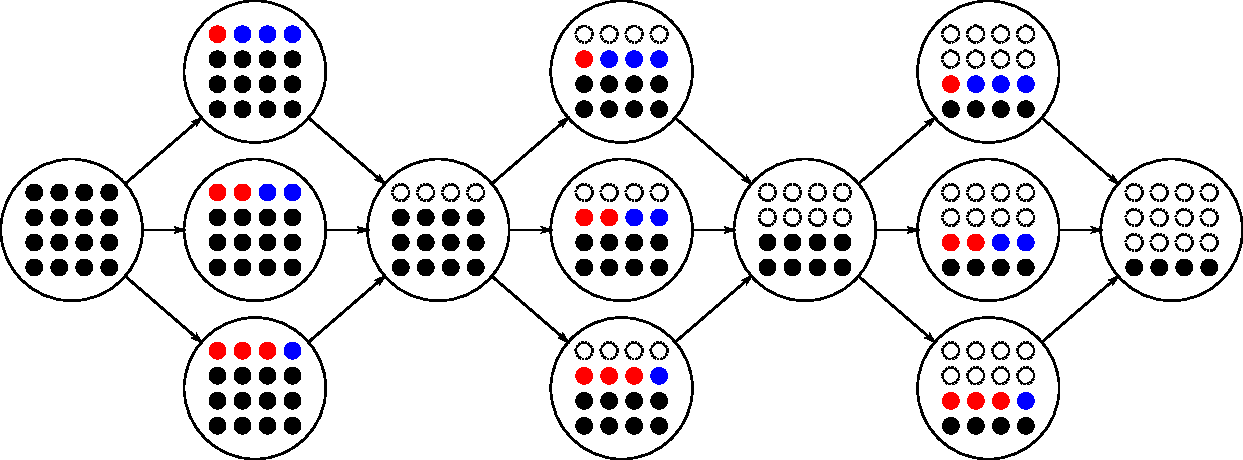
\includegraphics[width=\linewidth]{algo/nim/nim16.pdf}
\end{center}

\subsection*{Rapport avec l'informatique}

Comme pour le jeu de Nim, \textbf{un algorithme est une stratégie gagnante}
permettant de trouver la solution à un problème donné. Dans l'exemple précédent,
le problème était «~comment gagner au jeu de Nim ?~»

\encart{Pour aller plus loin}{
  On pourrait imaginer un cas plus général du jeu de Nim :

  \begin{itemize}
  \item Il y a $N$ objets sur la table au début du jeu \\ (pour notre version,
    $N=16$)
  \item Un joueur peut prendre jusqu'à $X$ objets à la fois \\ (pour notre
    version, $X=3$)
  \end{itemize}

  Quelles modifications doit-on apporter à notre stratégie gagnante pour qu'elle
  marche dans le cas général ?  }

\section*{Le coin de l'animateur}

L'objectif de cette activité est simplement d'introduire la notion d'algorithme
comme stratégie gagnante pour un problème donné.

\begin{itemize}
\item Commencez par jouer avec les participants, sans dire qu'il y a un truc. Si
  vous jouez bien, vous gagnerez à tous les coups.
\item Bien sûr, pour gagner, vous devez laisser votre adversaire commencer.
  S'il insiste pour ne pas commencer, vous pouvez toujours essayer de gagner en
  rattrapant la stratégie gagnante à la première erreur.
\item Si un participant connaît déjà la stratégie gagnante du jeu, il pourra
  vous remplacer pour jouer avec les autres participants.
\item Si vous n'êtes pas sûr d'appliquer correctement la stratégie gagnante,
  proposez un match en 3 --- ou en 5, en cas de coup dur ;) --- manches
  gagnantes.
\item Pour amener les participants à découvrir la stratégie gagnante, vous
  pouvez grouper les objets par 4, rendant ainsi l'astuce plus visible.
\end{itemize}


